\section{Baseline: Temporal Replication and Parallel Mining}
\label{sec:trm}
We resort to MapReduce (MR) as a general, parallel and scalable paradigm for GCMP pattern mining.
Since a GCMP pattern may cross multiple temporal segments, 
we cannot simply split the trajectory database into disjoint partitions and conduct parallel mining within each partition. Instead, we need certain data replication to guarantee that no matching patterns are missing.

We propose a framework named \emph{Temporal Replication and ParallelMining} (TRPM), 
as illustrated in Figure~\ref{fig:trm}. The mining procedure consists of 
two cycles of map-reduce jobs connected in a pipeline manner. In the first 
map-reduce cycle, input trajectories are grouped into snapshots and then clustered. 
In particular, object locations at the same timestamps form
a snapshot in the map-phase. In the reduce phase, objects in a snapshot
are clustered by the supplied clustering methods (e.g., DBSCAN or disk-based) in parallel.
The reducers finally output clusters of objects in each snapshot, 
represented by a list of $\langle t, S_t \rangle$ 
where $t$ is the timestamp and $S_t$ is a set of clustered object at snapshot $t$. 
The outputs will be fed into the second cycle of map-reduce jobs, whose details are presented in Algorithm~\ref{algo:trm_overview}. Intuitively, we first replicate each snapshot and each consecutive segment with $\eta$ snapshots is considered as one data partition. Then, a \emph{Line Sweeping} method is developed to discover GCMP within each partition in the reduce stage. The final patterns from all partitions are then stored into external storage (e.g, HDFS). In the following, we are interested to examine the minimum $\eta$ and introduce the \emph{Line Sweeping} algorithm in details.

\begin{figure*} [t]
\center
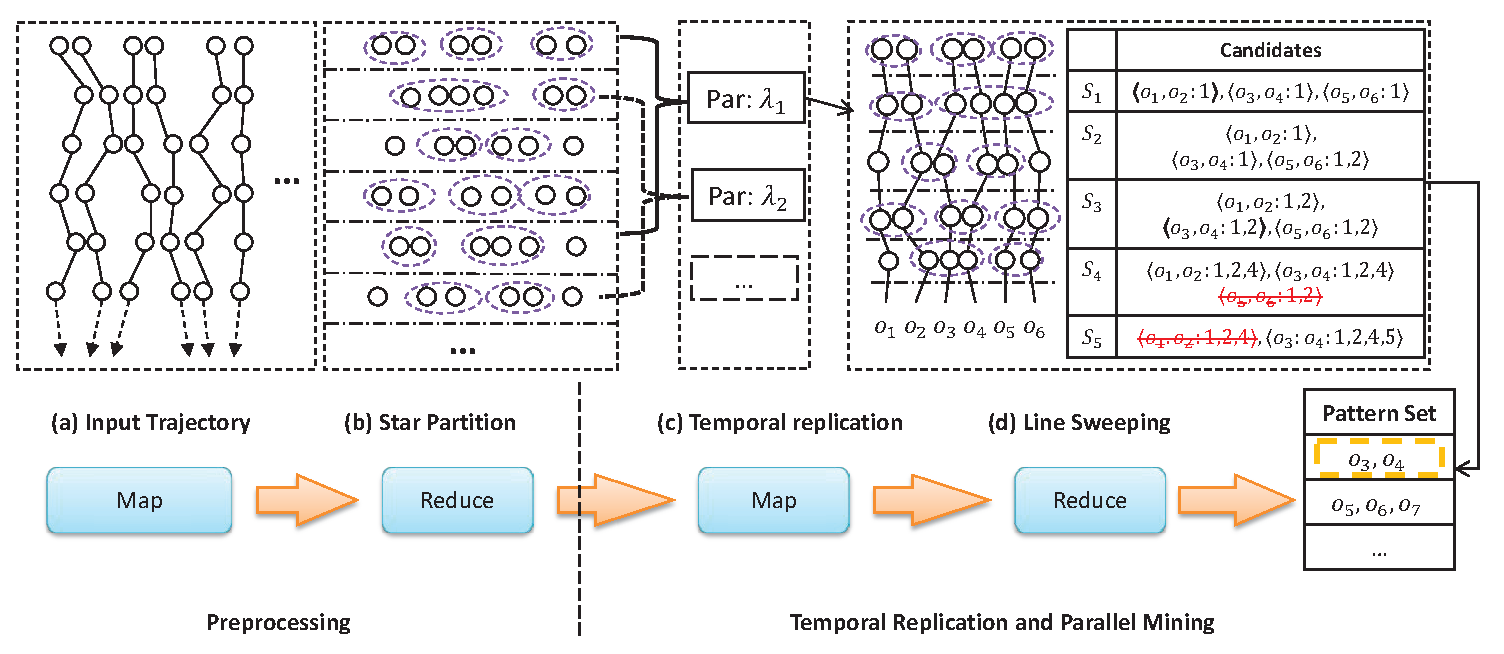
\includegraphics[width=\textwidth]{trm.eps}
\caption{Work flow of Temporal Replication and Mining. (a)(b) correspond to the first map-reduce cycle which clusters objects in each snapshot;  (c)(d) correspond to the second map-reduce cycle which uses temporal replication to mine GCMP in parallel.}
\label{fig:trm}
\end{figure*}


\begin{algorithm}
\caption{Temporal Replication and Parallel Mining}
\label{algo:trm_overview}
\begin{algorithmic}[1]
\Require list of $\langle t, S_t \rangle$ pairs
\State $\eta \gets (\lceil \frac{K}{L} \rceil -1)*(G-1)+2K-2$
\State {---Map Phase---}
\label{code:trm-map-start}
\ForAll{$\langle t, S_t \rangle$}
	\ForAll{$i \in 1...{\eta-1}$}
		\State emit a $\langle \max(t-i,0), S_t \rangle$ pair
	\EndFor  
\EndFor
\label{code:trm-map-end}
\State {---Partition and Shuffle Phase---}
\label{code:trm-par-start}
\ForAll{$\langle t, S \rangle$ pair} 
\State group-by $t$, emit a $\langle t, \lambda_t\rangle$
\State where $\lambda_t = \{S_t, S_{t+1}, .. S_{t+\eta-1}\} $
\EndFor
\label{code:trm-par-end}
\State {---Reduce Phase---}
\label{code:trm-red-start}
\ForAll{$\langle t,\lambda_t \rangle$}
\State lineSweepMining($\lambda_t$)
\label{code:trm-red-end}
\EndFor
\end{algorithmic}
\end{algorithm}

%\subsection{Temporal Replication}
In temporal replication, every partition
contains $\eta$ consecutive snapshots.
Therefore, determining $\eta$ is critical in ensuring the
correctness and efficiency of TRPM.
If $\eta$ is too small, some cross-partition patterns may be missed out. 
On the other hand, if $\eta$ is too large, the shuffle and reduce
stage of TRPM would incur expensive costs.
To guarantee the \emph{complete} discovery of all patterns, we enforce the
following statement on $\eta$: \emph{Let $T'$ be the \emph{shortest} 
valid subsequence (wrt. $K,L,G$) of a valid temporal sequence $T$. 
Then, $\eta$ needs to be the upper bound for all $T'$ among all valid temporal sequences to ensure the completeness.} 
Finding the \emph{minimum} $\eta$ is not
straightforward. We notice the minimum $\eta$ is related to the temporal
parameters $K,L,G$ by making the following observation on $G=1$:

\emph{
Let $T$ be an arbitrary valid temporal sequence. Since $G$ equals to 1,
$T$ can be represented as $T=(t_1, t_2,...,t_m)$, where
$t_i +1 = t_{i+1}$ and $m \geq K$. Let $T' = (t_1,...,t_k)$, $T'$ is the shortest
valid temporal sequence of $T$. Note that $T'$ is fully contained
in the partition $\lambda_{t_1} = \{S_{t_1},...,S_{t_k}\}$, therefore it can be
mined in $\lambda_{t_1}$. 
Since $T$ is an arbitrary valid temporal sequence, the minimum $\eta$ is thus $K$.
}

Inspired by the observation, we generalize the relationship between
the minimum $\eta$ and temporal parameters using the following theorem:
%
%
%Given any partition method, its correctness can be defined
%using \emph{completeness} and \emph{soundness} as follows: 
%
%\begin{definition}[Completeness and Soundness]
%Let a partition method $\mathbb{P}$ partitions a trajectory database $Tr$ 
%into segments, $Par_1,...,Par_m$. $\mathbb{P}$ is complete 
%if for every valid pattern $P$ in $Tr$, $\exists Par_i$ s.t. $P$ is valid in $Par_i$. 
%$\mathbb{P}$ is sound if for all patterns that are valid in any $Par_i$, they are also valid in $Tr$.
%\end{definition}

%Intuitively, \emph{soundness} avoids any false patterns in any partitions; while \emph{completeness}
%ensures no patterns are missed out by the partitions. In temporal replication, 
%the replication factor $\eta$ is critical. If $\eta$ is to small, such 
%partition may not be \emph{complete}. On the other hand, a large $\eta$ would incur
%expensive costs in the shuffle and reduce stages. Therefore, we need to find
%the \emph{minimum} $\eta$ such that the \emph{completeness} and \emph{soundness} are
%satisfied. Such an $\eta$ value is as stated in the following theorem:

\begin{theorem}
\label{THM:RP_ETA}
The minimum $\eta$ to ensure the completeness of the temporal replication is:
\[
   \eta = 
\begin{cases}
    (\lceil \frac{K}{L} \rceil -1)*(G-1)+2K -2, & \text{if } G \geq 2\\
    K,              & \text{if } G = 1
\end{cases}
\]
, where $K,L,G$ are the temporal parameters.
\end{theorem}

\begin{proof}
When $G = 1$, we have demonstrated $\eta=K$
in the above observation. When $G \geq 2$, we compute $\eta$ as follows:
any $T'$ can be viewed as $n$ consecutive segments with sizes $l_1,..,l_n$
and $n-1$ gaps with sizes $g_1,...,g_{n-1}$.
Since $\eta$ is the upper bond among all $T'$s, $\eta$ can be formulated 
as follows:
\begin{equation}
\eta = \max_{n,l_i,g_i} \{ \Sigma_{i=1}^{i=n} l_i + \Sigma_{i=1}^{i=n-1} g_i \}
\end{equation}
With the following constraints: (1)$\forall l_i, L \leq l_i \leq K-1$; (2)
$\forall g_i, 1 \leq g_i \leq G-1 $; (3) $\Sigma_{i=1}^{i=n} l_i \geq K$ and
(4) $\Sigma_{i=1}^{i=n-1}l_i  \leq K-1$. Constraints (1)(2)(3) due to the 
validity of $T'$ and $G\geq 2$ (4) is because $|T'|$ is minimum.
Based on (1)(3)(4), we can derive (5):  $n \in [1, \lceil \frac{K}{L} \rceil]$.
Constraints (1)-(5) form a convex polygon and $\eta$ is monotone
increasing wrt. $n, l_i, g_i$, therefore, the maximum value of $\eta$ is taken at the upper boundaries
where $g_i = G-1$, 
$\Sigma_{i=1}^{i=n-1}l_i = K-1$, $l_i = K-1$
and $n = \lceil \frac{K}{L} \rceil$. This leads to  $\eta = (\lceil \frac{K}{L} \rceil -1)*(G-1)+2K -2$.
\end{proof}

Based on the above theorem, during TRPM, every consecutive $\eta$ snapshots
form a partition. In particular, for every snapshot $S_t$, there is
a partition $\lambda_t=\{S_t,...,S_{t+\eta-1}\}$. With this partition strategy,
when discovering GCMPS in $\lambda_t$, we only need to keep the pattern candidates whose
object set are in $S_t$. This motivates to design an efficient 
\emph{line-sweep} mining (LSM) method for each partition. The intuition of LSM is 
to sequentially scan all snapshots. During scanning, a set of pattern candidates is maintained.
When all snapshots are scanned, the remaining candidates are the true patterns.
The detail of LSM is presented in Algorithm~\ref{algo:line-sweep}.
% To discover
%valid patterns from each partition, we design a \emph{line-sweep} mining (LSM) method as 
%shown in Algorithm~\ref{algo:line-sweep}. 
%The algorithm sequentially scans snapshots in a partition. 
%During the scan, it
A candidate set $C$ is maintained throughout the algorithm(line~\ref{code:ls-can-set}). $C$
is initialized by inserting clusters at $S_t$ (lines~\ref{code:ls-init-start}-\ref{code:ls-init-end}).
During scanning snapshot $S_j$, candidates in $C$ are joined with clusters at $S_j$. In
the join, a candidate grows its temporal sequence while potentially reduces its object set. After the join,
false patterns are deleted (line~\ref{code:ls-remove}). 
Note that the size of $C$ is always decreasing, therefore the complexity of LSM $\lambda_t$ is $O(\eta|S_t||\overline{S}|)$,where $|\overline{S}|$ is the average snapshot size in $\lambda_t$.

%It maintains a candidate set $C$ which contains potential patterns (line~\ref{code:ls-can-set}).
%The algorithm starts by inserting clusters at $S_t$ to $C$ (lines~\ref{code:ls-init-start}-\ref{code:ls-init-end}).
%Subsequently, when scanning $S_j$, clusters in $C$ are joined with clusters at $S_j$ to generate
%a new set of patterns $N$(lines~\ref{code:ls-join}). The valid new patterns 
%form a new candidate set $C$ and any invalid patterns are discarded(lines~\ref{code:ls-add} and~\ref{code:ls-remove}).


%$\eta$ is firstly determined based on pattern parameters.
%In the map phase, $\eta$ snapshots form a partition, followed by the reduce phase where 
%the line sweep algorithm is applied on each partition.

%MOVE THE PROOF TO APPENDIX

%In the Algorithm~\ref{algo:trm_overview}, 
%the partition size is chosen as $(\lceil \frac{K}{L} \rceil -1)*G+2K$. As stated in the following
%theorem, such a partition method is sound and complete.
%\begin{theorem}[Soundness and Completeness of Replication]
%\label{thm:replication_partition}
%Let $\mathbb{P}$ be as follows: for each snapshot $S_t$, create a partition $Par_t = \{S_t, ...,S_{t+(\lceil \frac{K}{L} \rceil - 1) *G+2K}\}$. Then $\mathbb{P}$ is sound and complete.
%\end{theorem}
%\begin{proof}
%The soundness of partition can be observed from the fact that each partition represents partial trajectories with consecutive snapshots, therefore patterns in a partition can be directly mapped back to original trajectories.
%Given a valid pattern $P$, let $T' \subseteq P.T$ be the subsequence of $P.T$ which conforms to $K,L,G$ with the smallest size. Note that there could be many qualified $T'$s.  
%Let the $i^{th}$ local-consecutive part of $T'$ be $l_i$ and let the $i^{th}$ gap of $T'$ be $g_i$. Then, the size of $T'$ can be written as $\Sigma_i (l_i + g_i)$. 
%Since $T'$ conforms to $K,L,G$, then $2K \geq \Sigma_i (l_i) \geq K$, $l_i \geq L$, $g_i \leq G$. Therefore, $\Sigma_i(l_i+g_i) \leq (\lceil \frac{K}{L} \rceil -1) *G+2K$. Thus ensuring each $Par_t$ to be of that size would capture at least one of the $T'$s, therefore the pattern $P$ would be valid in $Par_t$. This proves the completeness of the partitioning method.
%\end{proof}

%\subsection{Line Sweep Mining}
%Each job in the reduce phase handles a partition $\lambda_t$, 
%which contains $\eta$ snapshots starting from snapshot $S_t$. 
%We observe that within each partition, only the patterns whose object sets are contained in the first snapshot are necessary to be reported. %YOU CAN FORMALIZE THIS STATEMENT AS A LEMMA AND PROVIDES A RIGOROUS PROOF. 
%Therefore, we design a 
%\emph{line-sweep mining}(LSM) method in Algorithm~\ref{algo:line-sweep} to discover GCMPs. 
\begin{algorithm}
\caption{Line Sweep Mining}
\label{algo:line-sweep}
\begin{algorithmic}[1]
\Require $\lambda_t = \{S_t, ..., S_{t+\eta-1}\}$
\State{$C \gets \{\}$} \Comment{Candidate set} \label{code:ls-can-set}
\For{$c \in S_t$} 
\label{code:ls-init-start}
\State $C$.add($\langle c, t \rangle $)
\EndFor
\label{code:ls-init-end}
\ForAll{$j \in [t+1,t+\eta-1]$}
\State $C \gets S_{j} \oplus C$ \label{code:ls-join}
	\State{remove false candidates from $C$}
	\label{code:ls-remove}
\EndFor
\State{output true candidates in $C$}
\end{algorithmic}
\end{algorithm}


%\begin{figure}[h]
%\centering
%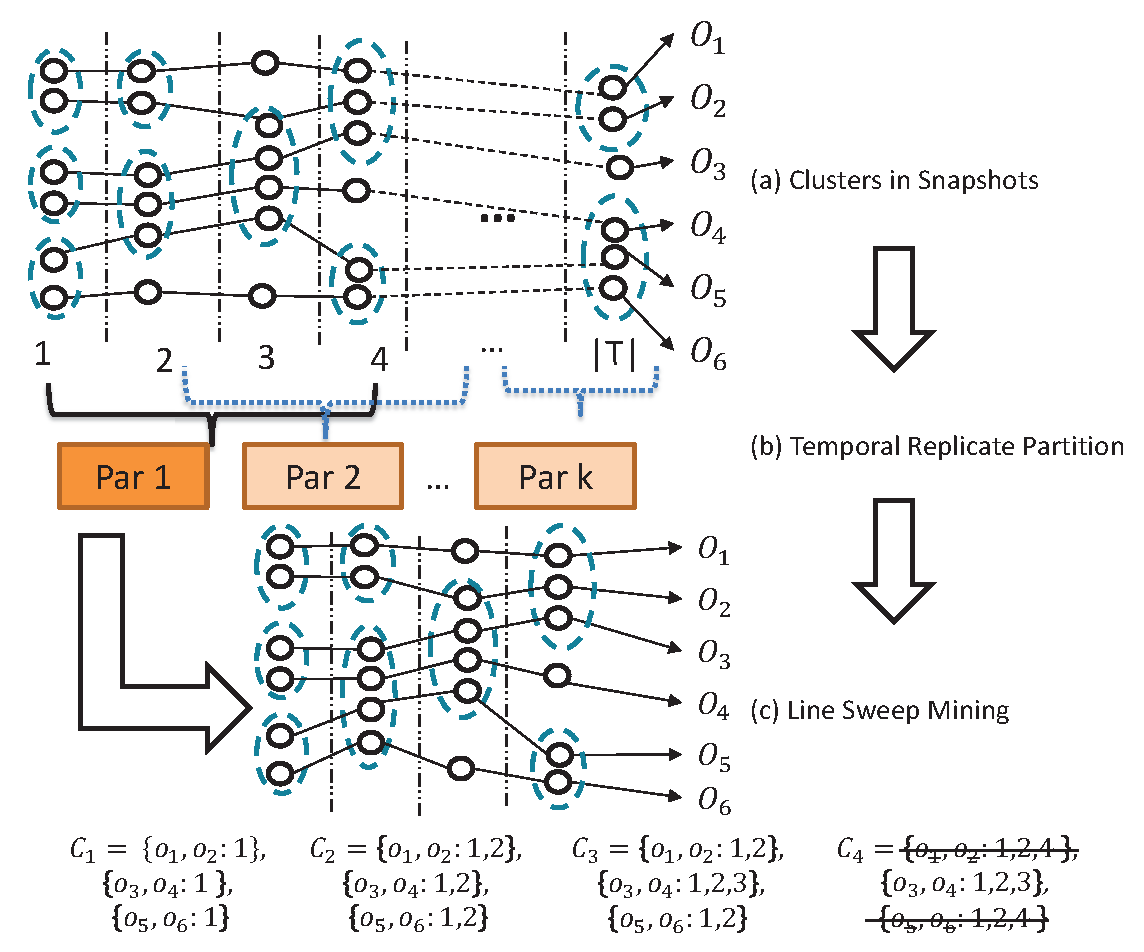
\includegraphics[width=0.5\textwidth]{trm_process.eps}
%\caption{Work flow of trajectory replication and mining}
%\label{fig:trm_process}
%\end{figure}


\begin{example}
We illustrate the work flow of TRPM method using Figure~\ref{fig:trm} (c)(d) with pattern
parameters $M=2, K=3, L = 2, G=2$. By Theorem~\ref{THM:RP_ETA}, $\eta$ is calculated
as $(\lceil \frac{K}{L} \rceil-1) *(G-1)+2K - 2 = 5$. Therefore, 
in Figure~\ref{fig:trm} (c), every $5$ consecutive snapshots are combined 
into a partition in the map phase. In Figure~\ref{fig:trm} (d), a line sweep
method is illustrated for partition $\lambda_1$. Let $C_i$ be the candidate set
during sweeping snapshot $S_i$.
Initially, $C_1$ contains patterns whose object set is in snapshot $S_1$.
As line sweeps, the patterns in $C_i$ grows. At snapshot $S_4$, the candidate
$\{o_5,o_6\}$ is removed. This is because the gap between its latest timestamp (i.e., $2$)
and the next scanning timestamp (i.e., $5$) is $3$, which violates the $G$ constraint.
Next, at snapshot $S_5$, the candidate $\{o_1,o_2\}$ is removed. This is
because its local consecutive timestamps $\{4\}$ has only size $1$,
which violates the $L$ constraint.
Finally, $\{o_3,o_4\}$ is the qualified pattern and is outputted. Note that the minimum $\eta$
under this setting is $5$. If $\eta$ is chosen as $4$, the pattern $\{o_3,o_4\}$ would be excluded. 
\end{example}


%
%Even though the TRM algorithm works in a parallel way, it requires to replicate the data $\eta$ times. 
%When $\eta$ is small, TRM perform good parallelism. However, wh
%
%When handling \emph{swarm}, \emph{group} and \emph{platoon} patterns, $\eta$ has to be set to $|\mathbb{T}|$ to guarantee correctness, resulting in very expensive data replication overhead. 
%%Handling those cases are equivalent to replicate the entire snapshots to each partition, 
%%which surrenders the benefit of parallelism.
Although TRPM works in a parallel way, we observe two inefficiencies. First, the
performance of TRPM largely relies on $\eta$ which further depends on pattern parameters.
When $\eta$ is large, the shuffle and reduce cost of TRPM is high. Second, 
the parallel execution of line sweep algorithm may discover the same pattern from
multiple partitions, which introduces redundant work. To resolve the two limitations,
we design a novel \emph{Star Partition and Mining} algorithm.